\chapter{Fundamentos Musicais}
	\label{ch:fundamentos}
Para compreensão do trabalho faz-se necessário a introdução de fundamentos musicais relacionados ao som, à síntese sonora, e ao processo criativo ligado a composição e improvisação musical.

\section{Som}
De acordo com \cite{med1996teoria} o som é a sensação produzida no ouvido pelas vibrações de corpos. Uma vibração põe em movimento o ar na forma de ondas sonoras que se propagam em todas as direções simultaneamente. Isso é similar ao jogar uma pedra dentro lago plano, a qual produz ondas circulares na superfície. 

Caso a vibração possua a forma de uma onda periódica, é considerada como uma vibração regular, o qual produz sons musicais como som de piano, violino. Caso contrário, a vibração irregular produz sons conhecidos como ruído, como som de avião, som de uma cadeira sendo arrastada. Na música ambos são usados, o som regular está presente nos instrumentos com notas bem definidas como piano, violão, enquanto os sons irregulares são usados geralmente em instrumentos de percussão como bateria.  

\subsection{Propriedades do Som}
O som independente da sua classificação, possui características básicas a frequência $f$, amplitude A, timbre e a duração.     

\begin{itemize}
	\item Frequência ($f$): também chamado de \textit{pitch}, é o número de ciclos por segundo numa onda periódica, a unidade de medida é \textit{Hertz} (Hz), ilustrado pela Figura \ref{fig:frequencia}. O valor de 100Hz indica que a vibração do som ocorre com a frequência de 100 ciclos por segundo.\cite{Miletto2004}. A frequência está relacionada diretamente com a percepção da altura do som, descrito em agudo ou grave, a Figura \ref{fig:zonasFrequencias} exemplifica. Dado dois sons com frequências $f_{a}$ e $f_{b}$ de valores 440Hz e 100Hz, respectivamente, o som de $f_{a}$ é mais agudo que o som de $f_{b}$, e $f_{b}$ é mais grave que $f_{a}$. 
		\begin{figure}[!htb]
			\centering
			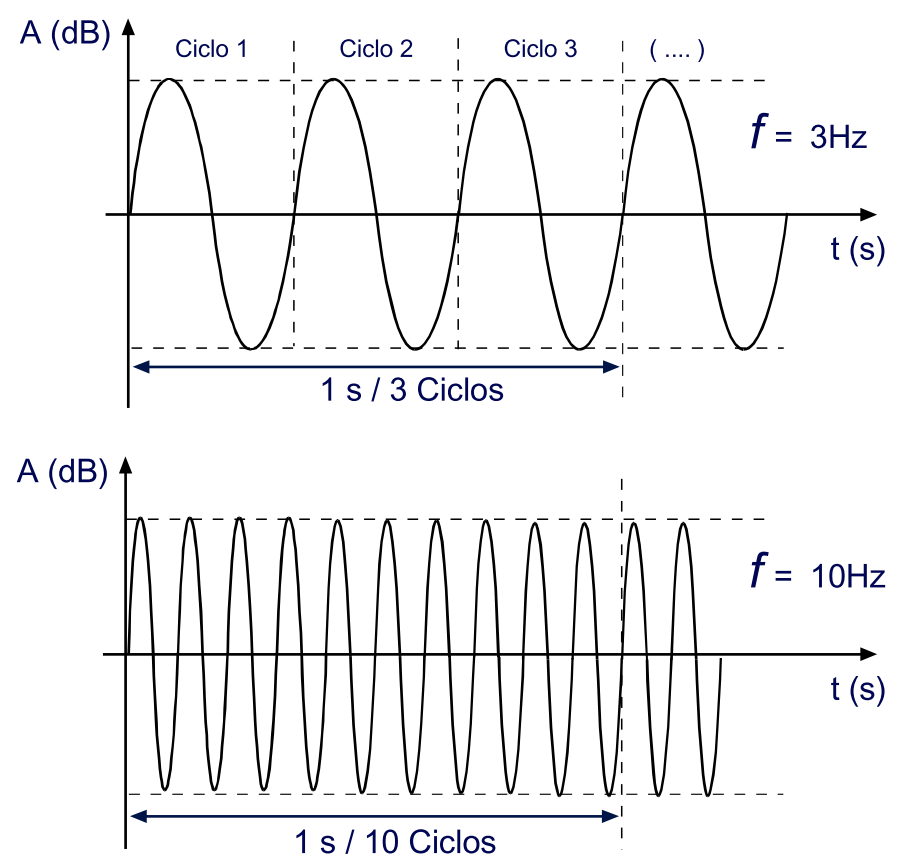
\includegraphics[height=6cm]{frequencia}
			\caption{São duas ondas periódicas senoidais em que o número de ciclos que decorrem ao longo de 1 segundo são respectivamente 3 e 10, pelo que as suas frequências serão 3Hz e 10Hz. Fonte: \cite{Barbosa1999}}
			\label{fig:frequencia}
		\end{figure} 
		\begin{figure}[!htb]
			\centering
			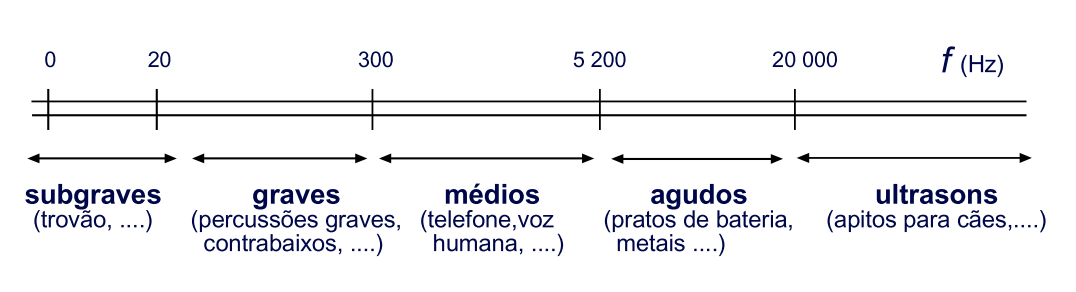
\includegraphics[height=4cm]{graveAgudo}
			\caption{O intervalo de frequências perceptíveis ao corpo humano, dividido em agudos e graves. Fonte: \cite{Barbosa1999}}
			\label{fig:zonasFrequencias}
		\end{figure}
	\item Amplitude (A): popularmente conhecido com volume, é a intensidade do som, ou seja, quanto maior a amplitude mais forte o som. A unidade de medida é \textit{Decibel} dB, \ref{fig:amplitude}.
		\begin{figure}[!htb]
			\centering
			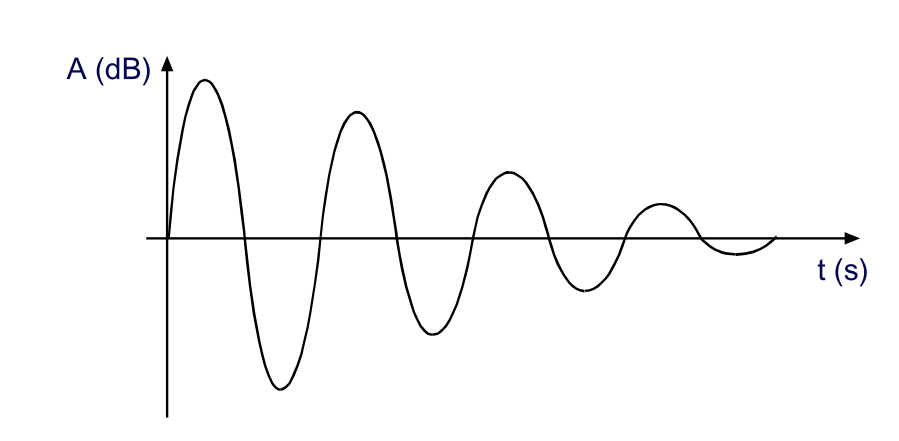
\includegraphics[height=4cm]{amplitude}
			\caption{Representação da amplitude de onda durante o tempo, onde inicialmente o som tem intensidade mais forte e com decorrer do tempo a amplitude diminui e som se torna mais fraco. Fonte: \cite{Barbosa1999}}
			\label{fig:amplitude}
		\end{figure}
	\item Timbre: é a qualidade do som que permite distiguir sons que possuem a mesma frequência e intensidade de instrumentos diferentes. É pelo timbre que sabemos se o som é proveniente de um violão, de um piano ou de uma voz humana. Isso ocorre porque as diferentes formas de ondas produzem sons diferentes, por exemplo na Figura \ref{fig:timbres}, as ondas arredondadas produzem sons suaves e as ponteagudas produzem sons brilhantes. Portanto, o timbre faz com que o som possa parecer aveludado, metálico, suave, brilhante. \cite{edgar1986}
		\begin{figure}[!htb]
			\centering
			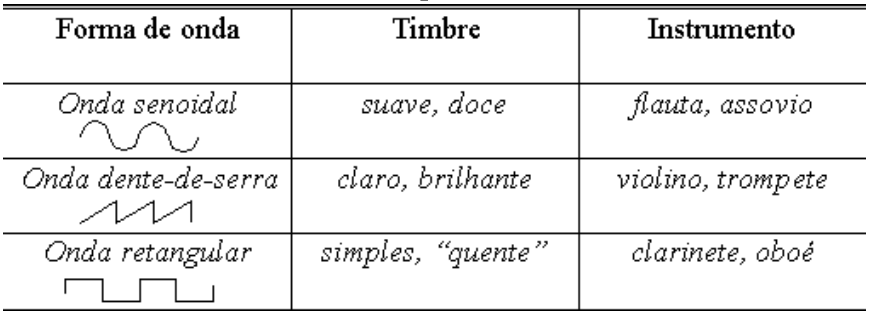
\includegraphics[height=4cm]{timbres}
			\caption{Exemplos de formas de ondas, característica do timbre e o som pertinente. Fonte: \cite{Miletto2004}}
			\label{fig:timbres}
		\end{figure}
		\item Duração ($t$): é o tempo de propagação da onda, ou seja, o tempo que um som dura até sua interrupção.
\end{itemize}

\subsection{Som digital}
Há vários tipos de sons e eles são percebidos no cotidiano, o som da voz de uma pessoa, do arrastar de movéis, do violão, do piano, dos computadores. Pensando nos sons citados é possível classificar o som como analógico (natural) ou digital (artificial). O som analógico é contínuo, desde modo todos os sons são percebidos de forma integral. O som analógico são dos instrumentos tradicionais como violino, flauta, bateria, voz. Enquanto o som/sinal digital é todo som gerado de forma artificial

O som digital foi o grande precursor para a computação musical \cite{roads1996computer}, ele tem como característica principal a não continuidade, ou seja, o som digital é representado de forma discreta ainda que isso seja imperceptível para o ouvido humano. É a base das áreas como o síntese de som e processamento de áudio. Um sinal é o som gerado por uma aplicação musical do computador, e esse sinal é entidade digital de mais baixo nível a ser considerada. 
% Ao nível da nota, uma nota (ou seja, pitch e duração) é a entidade musical mais baixa que é considerada, e tudo o mais é construído a partir daí. Nesse nível, além das representações convencionais de música, podemos estudar aspectos interessantes da chamada composição algorítmica, incluindo o uso de fractals, sistemas baseados em gramática, processos estocásticos e assim por diante. A partir desta base, também podemos estudar a análise harmônica e rítmica da música, embora isso não seja atualmente uma ênfase neste livro de texto. Haskell facilita a programação neste nível através de suas poderosas instalações de abstração de dados, funções de ordem superior e semântica declarativa
% Em contraste, no nível do sinal, o foco é o som real gerado em uma aplicação de música de computador e, portanto, um sinal é a entidade mais baixa que é considerada. O som é representado de forma concreta em um computador digital por uma amostragem discreta do sinal de áudio contínuo, a uma taxa suficientemente alta para que as orelhas humanas não possam distinguir o discreto do contínuo,
% \cite{Hudak2014}


\section{Síntese de Som}
A síntese sonora é uma técnica de geração de som utilizando equipamentos eletrônicos ou softwares, a partir do zero. O objetivo principal não é imitar sons existentes e sim criar sons totalmente novos. Um sintetizador, um instrumento musical eletrônico como a Figura \ref{fig:sintetizador}, tem a capacidade de emitir sons de piano, flauta, violão, mas o foco é criação de novos sons com timbres diferentes. Como um sintetizador, o computador também é um ferramenta a utilizar-se na síntese sonora.

\begin{figure}[!htb]
\centering
	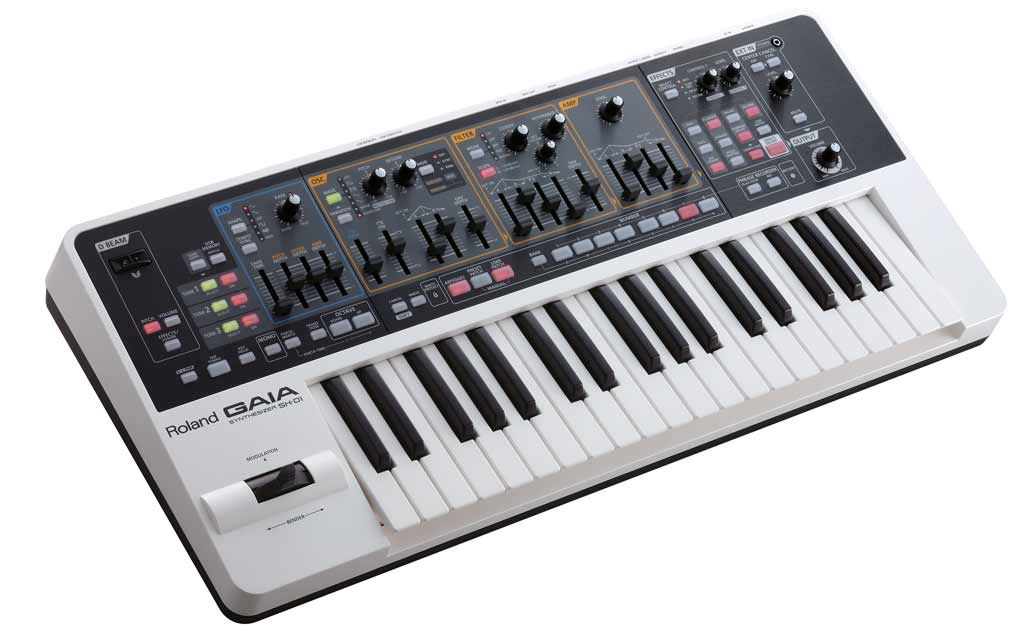
\includegraphics[height=4cm]{sintetizador}
	\caption{Exemplo de sintetizador: Roland Gaia. Fonte: Desconhecido.}
	\label{fig:sintetizador}
\end{figure}

Ao escolher técnicas para realizar a síntese há uma vasta gama de técnicas como síntese granular, aditiva, subtrativa entre outras.


-----------ESCREVER MAIS


\section{Processo Criativo}
O processo criativo é importante para o \textit{Live Coding} pela natureza perfomática da arte, fazendo-se necessário abordar sobre composição musical e improvisação.  

\subsection{Música}
De acordo com \cite{lacerda1966} a música é a arte dos sons, as principais partes da música são: melodia, ritmo, harmonia.

\begin{itemize}
	\item Melodia: o conjunto de sons dispostos em ordem sucessiva, é o tema da música, o qual capta a atenção do ouvinte;
	\item Harmonia: o conjunto de sons dispostos de forma simultânea que complementa a melodia;
	\item Ritmo: a ordem e proporção em que estão dispostos os son, definida também como a batida ou marcação do tempo.
\end{itemize} 

Esses elementos citados são básicos nas etapas de composição, sendo a melodia a mais importante da composição.

\subsection{Composição musical}
A composição musical tem como base o conhecimento do músico em relação a teoria musical e criatividade. É essencial o domínio de alguns fundamentos da teoria musical sobre a melodia, harmonia, ritmo, estilo musical, forma. A criatividade é muito influente na composição, ela está ligada com a ideias, sensibilidade do artista, ambiente onde este artista está inserido e entre outros fatores. A composição descrita aqui está ligada à criação de melodia, harmonia e definição dos instrumentos e não à criação de letra para uma música.  

O processo da composição acontece em quatro estágios: conscientização da ideia, concepção da forma, escolha do material sonoro definindo os sons e instrumentos presentes, e estruturação estabelecendo repetições e variações sonoras. % \cite{keylist}

Para um compositor é fundamental conseguir implementar sua criação de uma forma rápida e precisa, não por questões de produtividade, mas sim para poder reagir as suas ideias o mais próximo possível do tempo real \cite{Barbosa1999}. A tecnologia trouxe benefícios para o processo de composição musical. Os ambientes existentes para partitura e composição possibilitam que a melodia ou os arranjos criados possam ser ouvidos rapidamente com \textit{feedback}, logo após a inserção ou modificação da criação. Além de poder usar vários instrumentos diferentes na execução sem requerer a presença de um instrumentista. 	

----Ao enfocar os processos criativos envolvidos na composição musical, argumentam que “o escasso material que tem sido escrito sobre os processos criativos (em oposição ao produto) no domínio da composição têm sido quase exclusivamente na forma de relatos pessoais [...]”. Por conseguinte, são raros os estudos que investigam os fatores que inspiram os compositores na produção de suas obras


\subsection{Improvisação musical}	
A improvisação musical é a arte de compor e registrar ao mesmo tempo, onde o artista expressa em tempo real as suas ideias. É necessário ter domínio do instrumento e de teoria musical, de tal maneira que consiga assimilar rapidamente a ideia e colocá-la em prática. Muitos estilos musicais são baseados na improvisação durante uma performance, Jazz , Blues e música eletrônica são exemplos que possuem essa característica marcante.

	